

\documentclass[10pt,twocolumn,letterpaper]{article}

\usepackage{cvpr}
\usepackage{cite}
\usepackage{url}
\usepackage{graphicx}
\usepackage{clrscode}
\usepackage{tabularx}
\usepackage{amsmath}
\usepackage{array}
\usepackage{color}
\usepackage{balance}

\cvprfinalcopy
\ifcvprfinal\pagestyle{empty}\fi

\begin{document}

\title{An Implementation of the Active Contours without Edged model and the Logic Framework for Active contours on multi-channel images}

\author{Karim Ali and Sarah Nadi\\
\{karim, snadi\}@cs.uwaterloo.ca \\
David R. Cheriton School of Computer Science\\
University of Waterloo\\
}



\maketitle

\begin{abstract}
%\boldmath
The abstract goes here.
\end{abstract}



\section{Introduction}
Image segmentation or boundary detection is a very important problem in the area of Image Processing, and has received a lot of attention in the past. The
classical Active Contour model (or Snakes) proposed by Kass et al.~\cite{kass1988snakes} was the first model to use the idea of energy minimization to attract
a contour to the edges of the objects in an image. The Snakes model was very successful and variations of it very highly adopted later on
(E.g.~\cite{caselles1997geodesic}. Most of these models used the level set formulation for propagating fronts to evolve the curve. However, these models highly
depended on curvature motion (motion defined by the gradient of the curve) which led to poor performance in smoothed edges. To overcome these limitations, Chan
and Vese~\cite{chan2001active} propose an active contour model that does not depend on the edges (i.e the gradient) for propagating the curve to detect the
boundary of the object. Instead, they use a region-based approach based on the Mumford-Shah model~\cite{mumford1989optimal} to divide the image
into two regions: one inside the propagating curve, and one outside. The curve is at the boundary of the object if there is no difference in intensities inside
the curve as well as outside the curve.

The Active Contours without Edges model proposed by Chan and Vese (referred to as Chan-Vese model throughout the rest of this paper) was very successful in
detecting objects even in noisy or blurry images. It could also detect holes in objects which was usually a limitation in previous models. As an extension to
this work, Sandberg and Chan~\cite{sandberg2005logic} propose a logic framework (referred to as the Sandberg-Chan model throughout the rest of this
paper) that  performs logical operations on multiple images according to the curve propagation proposed in the Chan-Vese model. To achieve that, previous models
usually had two steps. They would either first segment the object in each channel separately then combine the segmented objects according to the logic operation
through bitwise operations (CITE) or they would apply logic operations to the different images then segment the resulting image (CITE). The first approach is
very costly, and the second approach requires a lot of prior knowledge about the intensities of each image. To overcome these drawbacks, the Sandberg-Chan
model is based on the idea of fitting a single contour to the object on all channels according to the logic operator, and based on regions.

In this paper, we report on our findings after implementing each of these models. We implemented both models in Matlab, and experimented with several images.
In this paper, we explain the details of our implementation as well as our results. The rest of this paper is organized as follows: Section~\ref{sec:bg} first
provides brief background about each of the two models implemented in this paper. Section~\ref{sec:implementation} then explains our implementation. In this
section, we explain how we implemented the models and any variations from the original papers. Section~\ref{sec:results} explains our evaluation criteria, and
presents the results we obtained. Section~\ref{sec:difficulties} discusses some of the difficulties we faced, and points out some BLA. Section~\ref{sec:concl}
concludes this paper by summarizing our findings.


\section{Background}
\label{sec:bg}

\subsection{Chan-Vese Model}
\label{sec:chan-vese}

The Chan-Vese model is a region based model for detecting objects in an image. It is based on a restriction Mumford-Shah model which divides an image into
regions and represents each region by a piecewise constant (the minimal partition problem). Figure~\ref{fig:region} shows what is meant by a region based
model. The figure shows an image $u_{0}$ which has a gray triangular object in it. The red curve, C, is the initial contour used to detect this object. The
main idea behind the model is that the curve divides the image into two regions: that inside the curve and that outside. Each region is represented by a
constant, c, which is the average intensity of the image values in each region. In order for the curve to fit the object, there must be no variation of the
intensities inside the curve as well as outside. In other words, this turns into a minimization problem of the difference of intensities inside (fitting term
one, $F_{1}$) plus those
outside (fitting term two, $F_{2}$). For example, in the figure, the point $(x_{1},y_{1})$ will have to be outside the curve in order to minimize the difference
between the points inside
the curve. Similarly, the point $(x_{4}, y_{4})$ will have to be inside the curve. Figure~\ref{fig:fitting} shows all the possibilities of the curve's fitting
according to its position with respect to the object.

More formally, the Euler-Lagrange equation (as derived in the original paper) representing the time motion of the curve C is shown in Equation~\ref{eqn:cvpde}.

\begin{equation}
\label{eqn:cvpde}
\frac{\partial{\phi}}{\partial{t}} = \delta_{\varepsilon}(\phi)[\mu\; \mathrm{div}(\frac{\bigtriangledown \phi}{|\bigtriangledown \phi|}) - \nu -
\lambda_{1}(u_{0} - c_{1})^2 +\lambda_{2}(u_{0} - c_{2})^2] 
\end{equation}

\begin{figure}[t]
\centering
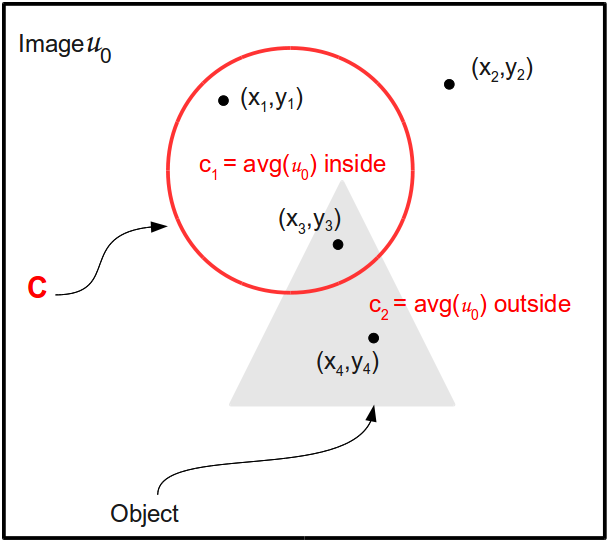
\includegraphics[width=6cm]{explaining.png}
\caption{Region Based Model}
\label{fig:region}
\end{figure}

(REST OF EQUATION HERE)

The parameter $\mu$ is a scaling parameter for the length of the curve represented in terms of curvature. The smalled $\mu$ is, the more the length of the curve
can increase without penalizing the minimization. This allows the model to detect smalled objects and holes. The larger $\mu$ is, the less freedom there is for
the curve to increase in length, and thus, it will only be able to detect larger objects. The parameter $\nu$ is also a scaling term for the area of the curve.
However, the authors do not use the area term in the Euler-Lagrange derivation, and always set $\nu$ to 0. It seems that $\mu$ is sufficient to scale the curve
according to the objects that need to be detected. Finally, $\lambda_{1}$ and $\lambda_{2}$ are weighting parameters for the forces inside the curve and
outside the curve respectively. Since we want to give both forces equal weight, the authors set $\lambda_{1} = \lambda_{2} = 1$ in all their experiments.



\subsection{Sandberg-Chan Model}
\label{sec:sandberg-chan}

The main goal of the Sandberg-Chan model~\cite{sandberg2005logic} is to perform logic operations on a combination of different images accurately and
efficiently. For example, finding the union of two images where different parts of the object are occluded in each image so that a complete object can be
obtained. In order to do that, they use the Chan-Vese model to detect objects, and simultaneously include the logic operations in the minimization problem.
Since they are using the Chan-Vese model, the problem must be viewed in terms of regions as well. Accordingly, they define the two main logic operations
(union and intersection) in terms of regions where the union of two images is the union of the insides of the curve with respect to the images plus the
intersection of the outsides of the curve with respect to the images. For example, Figure~\ref{fig:logic-op} (taken from the original paper) shows that the
union of $A_{1}$ and $A_{2}$ (in terms of its shape) can be obtained by taking the union of the insides of the object or the intersection of the outsides.
Similarly, the intersection of two images would be the intersection of the insides plus the union of the outsides. Thus, in order to obtain accurate results
irrespective of the object's intensity outside versus inside, we should consider \textit{both} the logical operation required for the region inside the object
as well as that outside.

\begin{figure}[t!]
\centering
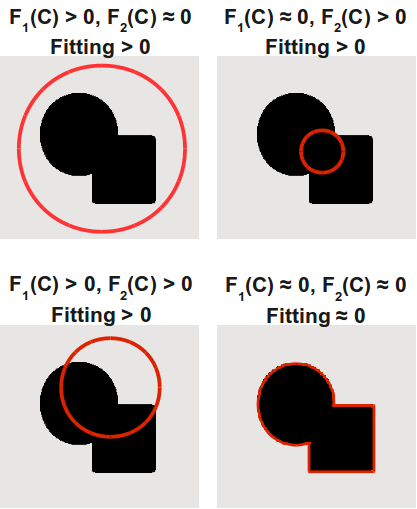
\includegraphics[width=6cm]{fitting.png}
\caption{Chan-Vese Curve Fitting}
\label{fig:fitting}
\end{figure}

More formally, the authors define two logic variables $z_{i}^{in}$ and $z_{i}^{out}$ to denote whether a point $(x,y)$ should be in the moving curve C or not
with respect to image i. Since we are trying to minimize the fitting of the curve, they use 0 to denote true and 1 to denote false (the reverse of the usual
convention. Following the Chan-Vese model, they represent each of the regions inside and outside the curve by a constant c. In this paper, they represent
$c_{in}$ as $c_{+}$ and $c_{out}$ as $c_{-}$. Equations~\ref{eqn:zin} and~\ref{eqn:zout} show how to calculate $z_{in}$ and $z_{out}$ respectively in terms of
the Chan-Vese model. We note here that in the original paper there was a typo in these equations where they divide by the maximum intensity of each image
instead of the maximum intensity squared. However, in order to have $z_{in}$ and $z_{out}$ have values from 0 to 1 that represent logic values, we need to
divide by the maximum intensity squared. The equations shown below have been corrected for that.

\begin{figure*}[t]
\centering
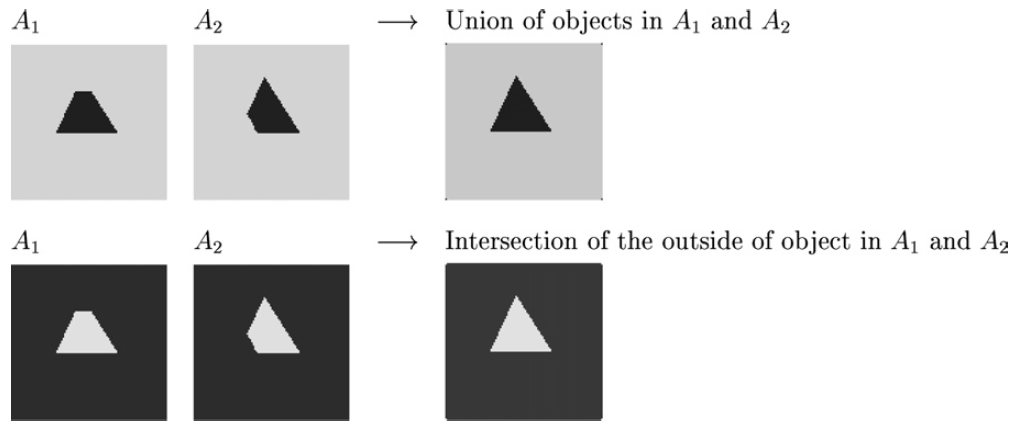
\includegraphics[width=12cm]{logicop.png}
\caption{Region Based View Union}
\label{fig:logic-op}
\end{figure*}

\begin{equation}
\label{eqn:zin}
z_{i}^{in}(u_{0}^{i},x,y,C) = \frac{|u_{0}^{i} - c_{+}^i|^2}{(max^{2}_{(x,y) \in u_{0}^{i}} u_{0}^i)^2}
\end{equation}

\begin{equation}
\label{eqn:zout}
z_{i}^{out}(u_{0}^{i},x,y,C) = \frac{|u_{0}^{i} - c_{-}^i|^2}{(max_{(x,y) \in u_{0}^{i}} u_{0}^i)^2}
\end{equation}

In order to perform logic operations on $z_{in}$ and $z_{out}$, the authors introduce interpolation functions that mimic the behavior of the regular truth
table, but for continuous values between 0 and 1. The union and intersection functions for two variables are shown in Equations~\ref{eqn:funion}
and~\ref{eqn:finters} respectively. These equations can be simply extended to any number of variables.

\begin{equation}
\label{eqn:funion}
f_{\cup} = (z_{1} . z_{2})^{1/2}
\end{equation}

\begin{equation}
\label{eqn:finters}
f_{\cup} = 1 = ((1 - z_{1}) .(1-  z_{2}))^{1/2}
\end{equation}

Based on these functions, the Euler-Lagrange equation for any logic operation is shown in Equation~\ref{eqn:svpde}. According to the desired logic operation,
$f_{in}$ and $f_{out}$ will be specified accordingly. For example, if we are doing the union of the images, then we will need to perform a union operation on
the insides. Thus, $f_{in}$ will be replaced by Equation~\ref{eqn:funion}. Similarly, we will need to do the intersection of the outsides so $f_{out}$ will be
replaced by Equation~\ref{eqn:finters}.

\begin{equation}
\label{eqn:svpde}
\frac{\partial{\phi}}{\partial{t}} = \delta(\phi)[\mu\bigtriangledown(\frac{\bigtriangledown \phi}{|\bigtriangledown \phi|})  - \lambda(f_{in}(z_{1}^{in}, ...,
z_{n}^{in}) - f_{out}(z_{1}^{out}, ..., z_{n}^{out})
\end{equation}

with the boundary condition

$\frac{\delta(\phi)}{|\bigtriangledown\phi|}\frac{\partial\phi}{\partial n^{\rightarrow}} = 0$

\section{Implementation}
\label{sec:implementation}

During implementation, we tried to stick to the authors' formulas and guidelines as much as possible. In this section we explain the choices we made regardless
implementation. For the chan-vese model, we used the PDE given in Equation 9 in the original paper~\cite{chan2001active} which is shown in
Equation~\ref{eqn:cvpde}.  We, first, tried to implement the delta dirac function, $\delta_{\varepsilon}\phi$, as defined in the paper. However, we did not
get non-zero values everywhere as indicated by the authors. Accordingly, we chose to use $|\bigtriangledown\phi|$ instead of the delta dirac function as this
was indicated as a valid alternative by the authors. To calculate $c_{1}$ and $c_{2}$, we simply calculated the mean of the values inside $\phi$ (specifically
where $\phi > 0$) and the mean of the values outside $\phi$ (specifically where $\phi < 0$) respectively. To actually solve the PDE, we chose to use an explicit
time stepping scheme for the finite difference discretization. That is, in each time step $\phi_{t} = \phi + \triangle t*force$. This was simpler to implement,
and although $\triangle t$ must be chosen carefully to satisfy the stability condition, we did not suffer from performance problems due to this restriction.

For the sandberg-chan model, we used the PDE given in original paper as well, and shown in Equation~\ref{eqn:svpde}. Again, we used $|\bigtriangledown\phi|$
instead of the dirac function. We calculated $z_{in}$ and $z_{out}$ according to Equations~\ref{eqn:zin, eqn:zout} shown above which have been corrected for
the typo in the original paper. For all other equations and calculations necessary in the model, we closely followed the original paper in our implementation.
We also used an explicit time stepping scheme in this model. 


\section{Experimental Results}
\label{sec:results}

In order to make sure we correctly implemented the models, we had several evaluation criteria. Table~\ref{tab:criteria} summarizes these criteria, and explains
the goals of each. Some of these criteria apply for both models, while other apply to one or the other. For the rest of this section, we proceed by presenting
our experimental results for both models. For each model, we proceed in the order of these criteria starting with the simplest
cases, and incrementally challenging the model. Unless otherwise stated, all the segmentation was performed on a gray scale version of the original image. All
the images in the Chan-Vese model were run on a BLA COMPUTER and all the images in the Sandberg-Chan model were run on a BLA computer.

\begin{table*}[h!t!]
\centering
\resizebox{\textwidth }{!}{
\begin{tabular}{ c | c |c}
\textbf{Criteria} & \textbf{Goal} & \textbf{Applies to Model}\\
\hline\hline
Detecting Boundaries & Ability to correctly detect object boundaries of simple objects& Both Models\\
\hline
Curve Position & Ability to correctly detect object boundaries irrespective of the initial curve position & Both Models\\
\hline
Detecting Holes & Ability to detect holes in objects, and not simply stop on outside boundary & Both Models\\
\hline
Blurred Images & Ability to correctly (as much as possible) detect object boundaries in blurred images & Both Models\\
\hline
Noisy Images & Ability to correctly (as much as possible) detect object boundaries in noisy images & Both Models\\
\hline
Union Operator & Ability to correctly obtain the union of two or more images & Sandberg-Chan\\
\hline
Intersection Operator & Ability to correctly obtain the intersection of two or more images & Sandberg-Chan\\
\hline
Complement & Ability to correctly obtain the union or intersection of two or more images containing complements & Sandberg-Chan\\
\hline
Parameter Settings & Ability to respond correctly to the different parameter settings & Both Models\\
\end{tabular}
}
\centering
\caption{Evaluation Criteria}
\label{tab:criteria}
\end{table*}

\subsection{Chan-Vese Model Results}

We present the results from the Chan-Vese model in this section, and show which criteria were met and which were not. Unless otherwise specified, we set
$\lambda_{1} = \lambda_{2} = 1$.

\subsubsection*{Successful Detection of Boundaries}

Figure~\ref{fig:cv_eg1} shows that the implemented model can successfully detect object boundaries in a simple image. In this case, the evolving curve was
successfully able to detect the boundaries of both objects. Figure~\ref{fig:cv_eg2} shows a slightly more complicated example where the evolving contour
successfully detects the contour of the brain. Note that there is a tiny area to the bottom left of the brain that was also successfully detected. To ensure
that open boundaries (e.g. lines) can also be detected, we used an image with several shapes shown in Figure~\ref{fig:cv_eg8};


\begin{figure*}[t]
\centering
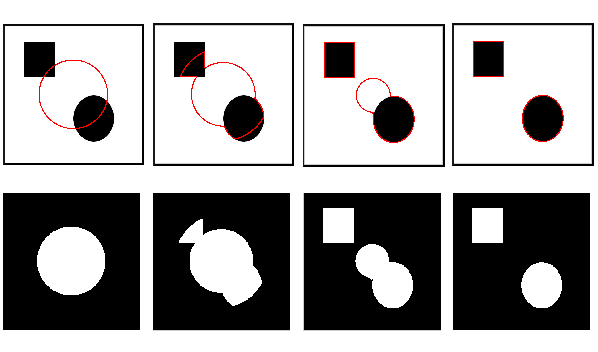
\includegraphics[width=12cm]{cv_eg1.png}
\caption{Successful detection of object boundaries. Top: the evolving curve (in red) over time where the first image shows the initial contour.
Bottom: evolving segmentation over time until the objects are detected. Size = 300 x 300, $\phi_{0}(x,y) = - \sqrt{(x - 150)^2 + (y - 150)^2)} + 75$, $\mu =
0.01$, no reinitialization, cpu = 2.9s, 7 iterations.}
\label{fig:cv_eg1}
\end{figure*}

\begin{figure*}[t]
\centering
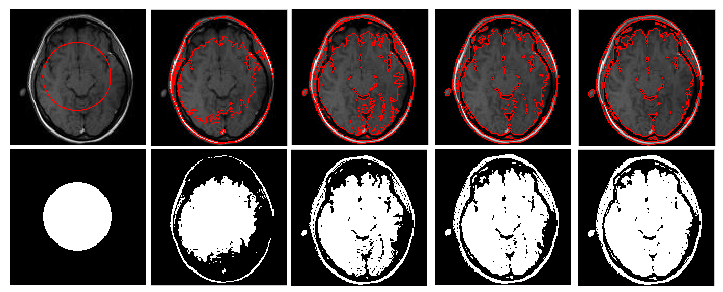
\includegraphics[width=12cm]{cv_eg2.png}
\caption{Successful detection of object boundaries. Top: the evolving curve (in red) over time where the first image shows the initial contour.
Bottom: evolving segmentation over time until the object is detected. Size = 131 x 131, $\phi_{0}(x,y) = - \sqrt{(x - 65.6)^2 + (y - 65.5)^2)} + 32.8$, $\mu =
0.01$, no reinitialization, cpu = 1.95 s, took 7 iterations.}
\label{fig:cv_eg2}
\end{figure*}

\begin{figure*}[t]
\centering
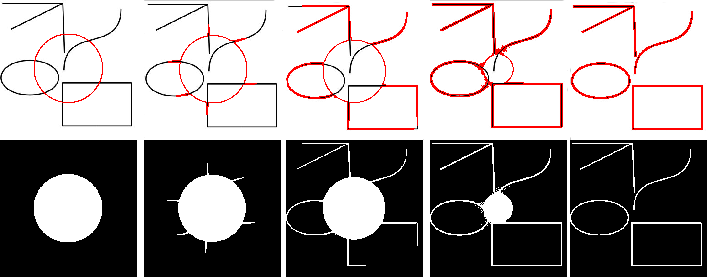
\includegraphics[width=12cm]{cv_eg8.png}
\caption{Successful detection of object with open boundaries. Top: the evolving curve (in red) over time where the first image shows the initial contour.
Bottom: evolving segmentation over time until the object is detected. Size = 300 x 300, $\phi_{0}(x,y) = - \sqrt{(x - 150)^2 + (y - 150)^2)} + 75$, $\mu =
0.01$, no reinitialization, cpu = 5.19 s, took 11 iterations.}
\label{fig:cv_eg8}
\end{figure*}


\subsubsection*{Independence of Initial Curve Position}

To ensure that the position of the curve does not affect the final segmentation, we tested two other positions for the initial curve for the same brain image
used in Figure~\ref{fig:cv_eg2}. In Figure~\ref{fig:cv_eg2}, the initial contour was completely overlapping the object. Accordingly, we tried two other
positions. The first one is shown in Figure~\ref{fig:cv_eg3} where the initial contour only partially overlaps with the object. The second one is shown in
Figure~\ref{fig:cv_eg4} where the initial contour does not overlap the object in any part. Visually, the obtained segmentation was the same with a slightly
higher number of iterations and CPU time. In all three cases, the brain was correctly segmented. We compared the area segmented as the brain in each case to
make sure the same segmentation was obtained, and in each case, we got the same area of 0.5268. Note, however, that when part of the curve lies outside the
object, the definition of inside and outside changes since the curve becomes an open curve at one point. This should not make a difference as long as the
contour lies correctly at the boundaries of the object. 

\begin{figure*}[t]
\centering
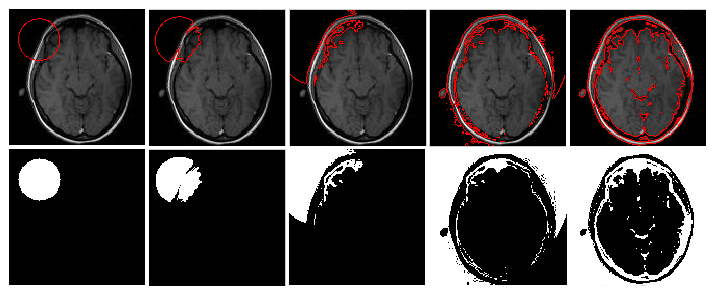
\includegraphics[width=12cm]{cv_eg3.png}
\caption{Initial curve position partially overlapping object. Top: the evolving curve (in red) over time where the first image shows the initial contour.
Bottom: evolving segmentation over time until the object is detected. Size = 131 x 131, $\phi_{0}(x,y) = - \sqrt{(x - 30)^2 + (y - 30)^2)} + 20$, $\mu =
0.01$, no reinitialization, cpu = 2.26 s, took 9 iterations.}
\label{fig:cv_eg3}
\end{figure*}

\begin{figure*}[t]
\centering
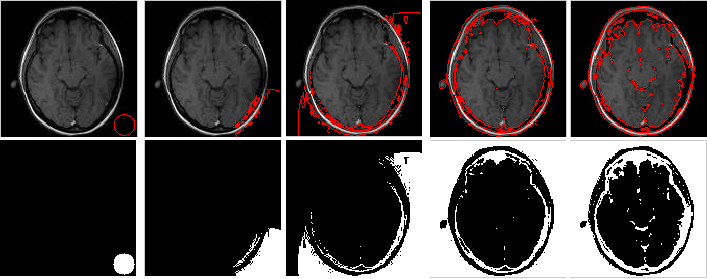
\includegraphics[width=12cm]{cv_eg4.png}
\caption{Initial curve position not overlapping any area of the object. Top: the evolving curve (in red) over time where the first image shows the initial
contour.Bottom: evolving segmentation over time until the object is detected. Size = 300 x 300, $\phi_{0}(x,y) = - \sqrt{(x - 120)^2 + (y - 120)^2)} + 10$,
$\mu =0.01$, no reinitialization, cpu = 2.01 s, took 9 iterations.}
\label{fig:cv_eg4}
\end{figure*}

\subsubsection*{Successful Detection of Holes}

In order to make sure the contour does not simply stop at the outside boundary of an object and ignore any details inside such as holes, we tried two donut
images. Figure~\ref{fig:cv_eg5} shows how the curve is able to detect the hole in the donut. Additionally, it is able to detect the various sprinkles on it.
We note that the bottom right boundary is not very exact, and this is because the lighting effect in the image makes the intensity of this area very close to
that of the background This is a known drawback of the Chan-Vese model since it only divides the image into two regions, and requires a big variation in
intensities for the curve to change. Another example showing this limitation is shown in Figure~\ref{fig:cv_eg7} where the flower parts with very low
intensities are not detected. We will show that we can overcome this limitation with the Sandberg-Chan model for this particular example.
Figure~\ref{fig:cv_eg6} shows that multiple holes in an image can also be successfully detected.

\begin{figure*}[t]
\centering
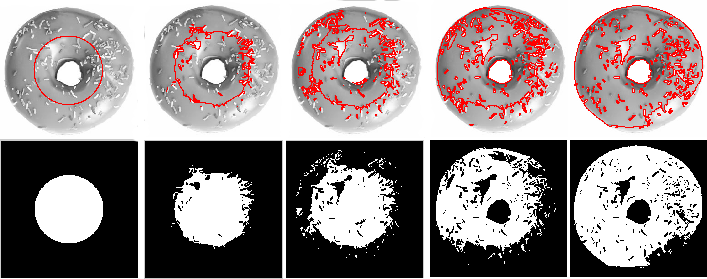
\includegraphics[width=12cm]{cv_eg5.png}
\caption{Successful detection of holes.  Top: the evolving curve (in red) over time where the first image shows the initial
contour.Bottom: evolving segmentation over time until the object is detected. Size = 131 x 131, $\phi_{0}(x,y) = - \sqrt{(x - 65.5)^2 + (y - 65.5)^2)} + 32.8$,
$\mu =0.01$, no reinitialization, cpu = 8.12 s, took 12 iterations.}
\label{fig:cv_eg5}
\end{figure*}

\begin{figure*}[t]
\centering
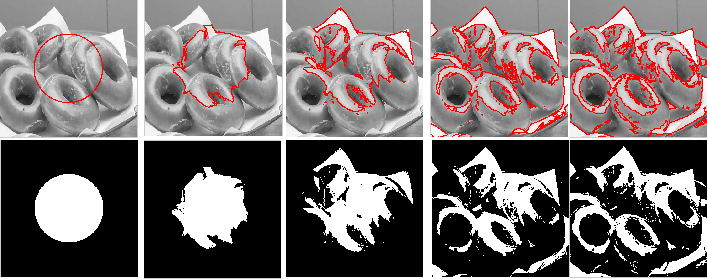
\includegraphics[width=12cm]{cv_eg6.png}
\caption{Successful detection of multiple holes.  Top: the evolving curve (in red) over time where the first image shows the initial
contour.Bottom: evolving segmentation over time until the object is detected. Size = 300 x 300, $\phi_{0}(x,y) = - \sqrt{(x - 150)^2 + (y - 150)^2)} + 75$,
$\mu =0.01$, no reinitialization, cpu = 15.07 s, took 23 iterations.}
\label{fig:cv_eg6}
\end{figure*}

\begin{figure*}[t]
\centering
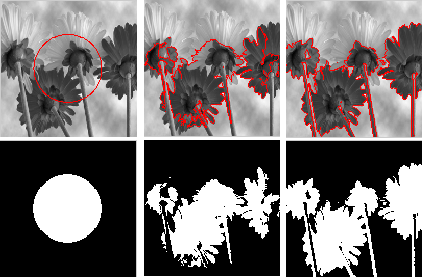
\includegraphics[width=12cm]{cv_eg7.png}
\caption{Inability to detect low intensities that have not much variation from their background.  Top: the evolving curve (in red) over time where the first
image shows the initial
contour.Bottom: evolving segmentation over time until the object is detected. Size = 300 x 300, $\phi_{0}(x,y) = - \sqrt{(x - 150)^2 + (y - 150)^2)} + 75$,
$\mu =0.01$, no reinitialization, cpu = 1.35 s, took 6 iterations.}
\label{fig:cv_eg7}
\end{figure*}

\subsubsection*{Reasonable Performance with Blurred Images}

Figure~\ref{fig:cv_eg9} shows how the contour behaves in a blurry image. The photographer was successfully detected. Additionally, other objects in the image
such as the tripod were found. However, objects with a very light intensity were again not detected.

\begin{figure*}[t]
\centering
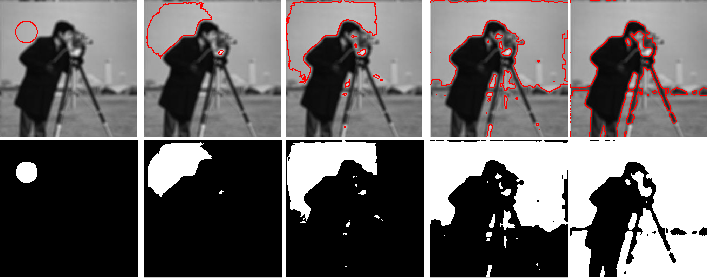
\includegraphics[width=12cm]{cv_eg9.png}
\caption{Ability to detect contours in blurry images.  Top: the evolving curve (in red) over time where the first
image shows the initial
contour.Bottom: evolving segmentation over time until the object is detected. Size = 255 x 255, $\phi_{0}(x,y) = - \sqrt{(x - 127.5)^2 + (y - 127.5)^2)} +
63.75$, $\mu =0.01$, no reinitialization, cpu = 5.41 s, took 15 iterations.}
\label{fig:cv_eg9}
\end{figure*}

\subsubsection*{Reasonable Performance with Noisy Images}

Figure~\ref{fig:cv_eg10} shows how two objects in a noisy image were successfully detected. In this image, we added Gaussian noise with mean zero and 0.01
variance using Matlab's built-in noise function. The image shows that although some of the noise was detected in intermediate iterations, the contour continued
to evolve until it was only surrounding the desired objects. Unfortunately, the effect of noise was not completely ignored in all cases. For example,
Figure~\ref{fig:cv_eg11} shows that for the same image, but with 'salt \& pepper' noise, the noise was detected as objects. This should not have been the case
since we used a large value $\mu = 5$ for the length scaling parameter. However, for some reason, varying $\mu$ did not have the intended effect as explained
in the next section. 

\begin{figure*}[t]
\centering
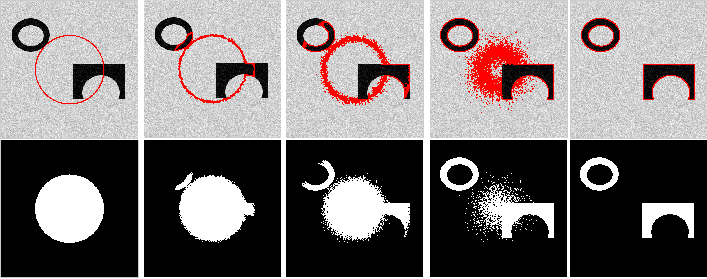
\includegraphics[width=12cm]{cv_eg10.png}
\caption{Ability to detect contours in an image with Gaussian noise.  Top: the evolving curve (in red) over time where the first
image shows the initial
contour.Bottom: evolving segmentation over time until the object is detected. Size = 300 x 300, $\phi_{0}(x,y) = - \sqrt{(x - 150)^2 + (y - 150)^2)} +
75$, $\mu =0.01$, no reinitialization, cpu = 4.4 s, took 7 iterations.}
\label{fig:cv_eg10}
\end{figure*}

\begin{figure*}[t]
\centering
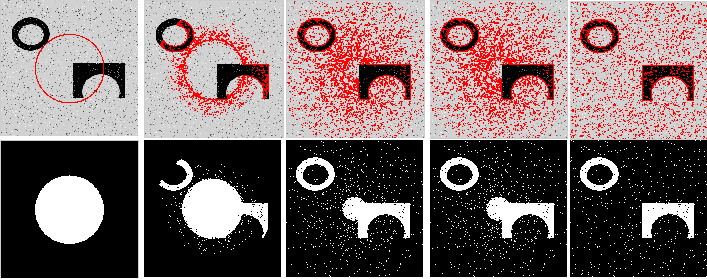
\includegraphics[width=12cm]{cv_eg11.png}
\caption{Same image as Figure~\ref{fig:cv_eg10}, but with 'salt \& pepper' noise. Noise was still detected despite increasing $\mu$.  Top: the evolving curve
(in red) over time where the first
image shows the initial
contour.Bottom: evolving segmentation over time until the object is detected. Size = 300 x 300, $\phi_{0}(x,y) = - \sqrt{(x - 150)^2 + (y - 150)^2)} +
75$, $\mu = 5$, no reinitialization, cpu = 12.27 s, took 7 iterations.}
\label{fig:cv_eg11}
\end{figure*}

\subsubsection*{Successful Response to Parameter Settings}

There are mainly three parameters in this model that can be varied: $\mu, \lambda_{1}, \lambda_{2}$. We would usually want both $\lambda_{1}$ and $\lambda_{2}$
to be equal to 1 to indicate that we care both about the difference of intensities inside and outside. A smaller weighting for one of them would mean that we
would ignore some of the variances in intensities in this area. A larger weighting means that we are magnifying the difference in intensities in that area
(i.e. we want to detect any minor changes). We show an example of these variations in Figure~\ref{fig:cv_eg12} where we vary
$lambda_1$ and $\lambda_2$. When we set $\lambda_1 = 0.2$ and $\lambda_2 = 1$, less details within the interior of the brain is detected. When
we set $\lambda_1 = 2$ and $\lambda_2 = 1$, we can see that more details within the brain are detected. When we set $\lambda_1 = 5$, and $\lambda_2 = 0.01$ (a
very extreme case), we can see that parts of outside boundaries are not well detected, while many details are detected within the brain.

\begin{figure*}[t]
\centering
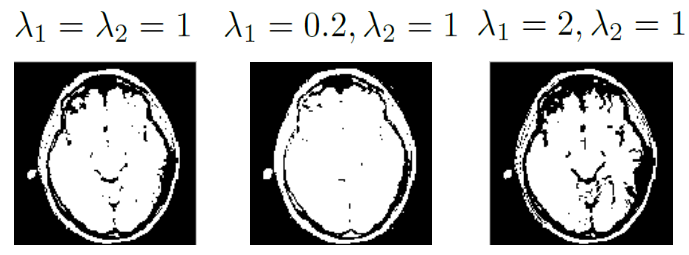
\includegraphics[width=12cm]{cv_eg12.png}
\caption{Effect of varying $\lambda_1$ which controls how much details are detected inside the contour. The figure shows the segmentation in each case.}
\label{fig:cv_eg12}
\end{figure*}

The second parameter, $\mu$ controls how much we allow the length of the curve to increase. If $\mu$ is small, it means that the curve length can increase to
detect multiple smaller objects without penalizing our minimization problem. On the other hand if $\mu$ is large, it means that any change in the curve length
will be scaled up, and thus will limit the curve expansion to keep the force to a minimum. Unfortunately, we were not able to see this effect in our
experiments. We tried varying increasing $\mu$ to be able to detect groupings of objects instead of the individual objects, but the segmentation was invariant
to $\mu$. We give more details about how we tried to handle this, and why we believe it is not working in Section~\ref{sec:difficulties}.

\subsection{Sandberg-Chan Model Results}

For the Sandberg-Chan model, the successful detection of boundaries criteria is implicitly 



\subsubsection*{Successful Detection of Boundaries}

\subsubsection*{Independence of Initial Curve Position}

\subsubsection*{Successful Detection of Holes}

\subsubsection*{Reasonable Performance with Blurred Images}

\subsubsection*{Reasonable Performance with Noisy Images}

\subsubsection*{Union}

\subsubsection*{Intersection}

\subsubsection*{Complement}

\subsubsection*{Successful Response to Parameter Settings}

\subsubsection*{Other Tests}

\section{Difficulties and Discussion}
\label{sec:difficulties}

\section{Conclusion}
\label{sec:concl}
The conclusion goes here.




\bibliographystyle{IEEEtran}

\bibliography{references}



% insert where needed to balance the two columns on the last page with
% biographies
%\newpage

\end{document}



